% Journal of Biomechanics - submission manuscript
% Double-spaced with continuous line numbers, per the Guide for Authors.
\documentclass[12pt]{article}

\usepackage[letterpaper,margin=1in]{geometry}
\usepackage{times}
\usepackage{amsmath}
\usepackage{graphicx}
\usepackage{booktabs}
\usepackage[round,authoryear]{natbib}
% hyperref/url are unavailable in this TeX install; URLs render as plain text.
\providecommand{\url}[1]{#1}

% setspace/lineno/caption are not in this TeX installation; double spacing is
% set directly. Line numbers must be enabled before submission (Overleaf has
% lineno): add \usepackage{lineno} and \linenumbers to this preamble.
\renewcommand{\baselinestretch}{1.9}\normalsize

\title{\textbf{Device-normalised geometry for muscle architecture\\
measurement in B-mode ultrasound}}
\author{Colton Downing\\[2pt]
\normalsize University of Southern California, Los Angeles, CA, USA}
\date{}

\begin{document}
\maketitle

\noindent\textbf{Word count (Introduction through Discussion):} approximately 2{,}900\\
\textbf{Conflict of interest:} none declared.

\vspace{1em}
\hrule
\vspace{1em}

\section*{Abstract}

Automated estimation of muscle architecture from B-mode ultrasound is
established, but existing tools assume a known and consistent acquisition: one
device, one export convention, and an operator-supplied spatial scale. We
address the case where none of that holds. Given only unlabelled screenshots
from six different ultrasound systems, with no metadata and no stated scale, we
recover pennation angle (PA), fascicle length (FL) and muscle thickness (MT)
entirely from the image.

Two corrections carry the result, and both are derived rather than fitted.
First, two of the six screenshot layouts are horizontally resampled exports in
which a transducer aperture is displayed across a width inconsistent with the
depth axis, so image pixels are not square; angles measured in pixel
coordinates on those devices are systematically wrong. We compute the aspect
ratio from published aperture specifications (Juniper 12L3, $R \approx 1.12$;
Lumify L12-4, $R \approx 0.84$) and resample to square physical pixels before
any geometry is evaluated. Second, the conventional fascicle-length estimator,
which extends a detected fascicle fragment to both aponeurosis lines, is exact
only when the aponeuroses are parallel. When they converge with half-angle $h$,
that chord exceeds $\mathrm{MT}/\sin\gamma$ by a factor
$1/(1-\cot^{2}\gamma\tan^{2}h)$. We show empirically that expert raters do not
reproduce this convergence-dependent inflation, and that a bisector-referenced
estimator reduces the bias spread across two anatomically distinct datasets
from six percentage points to one, permitting a single scalar calibration to
transfer between muscles.

On a 35-image benchmark with seven independent expert raters, the method scores
0.196 under the UMUD error formula against the seven-rater consensus, compared
with 0.331 for DL\_Track\_US, 0.409 for SMA, and a leave-one-out median of 0.264
for an individual expert rater. On an independent 167-frame dynamic sequence of
a different muscle, fascicle-length error is 1.82~mm using a calibration
constant fitted only on the static benchmark.

\vspace{0.5em}
\noindent\textbf{Keywords:} musculoskeletal ultrasound; muscle architecture;
fascicle length; pennation angle; image calibration

\newpage
\section{Introduction}

Muscle architecture --- the pennation angle of fascicles relative to the line of
action, their length, and the thickness of the muscle belly --- determines
force--velocity behaviour and is tracked clinically to monitor atrophy,
rehabilitation and training adaptation. These quantities are most often measured
by hand in ImageJ or FIJI, a procedure that is slow and, critically, not
reliable: for novice raters, within-rater intraclass correlations for manual
fascicle length have been reported as low as 0.00--0.30, against 0.90--0.99 for
a semi-automated algorithm \citep{frontiers2025}.

Deep-learning approaches have addressed this. \citet{cronin2020} trained U-Net
architectures to segment fascicles and aponeuroses, reporting agreement with
manual analysis within approximately 2.1~mm in FL. That work was substantially
extended and packaged as DL\_Track\_US \citep{ritsche2022}, now the standard
open-source tool in this domain, with reported mean differences against manual
analysis of $-2.4$~mm in FL, $0.6^{\circ}$ in PA and $-0.6$~mm in MT
\citep{ritsche2024}.

These systems share an assumption that limits their deployment: a known
acquisition. The spatial scale is supplied by the operator, the device is fixed,
and the image geometry is trusted. We consider the opposite case. The UMUD
Challenge provides 309 test images as screenshots from six different ultrasound
systems, with no metadata, no stated scale, and no indication of which device
produced which image. Everything required to convert pixels into millimetres ---
and, as we show, the pixel aspect ratio itself --- must be recovered from the
image.

This paper makes two methodological contributions. The first is a device
normalisation stage that identifies the scanner family, reads the on-screen
depth ruler, and corrects lateral anisotropy in resampled screenshot exports, a
correction absent from the reference implementations and one that materially
alters every measured angle on two of six layouts. The second is a geometric
analysis of the fascicle-length estimator showing that the conventional form
inherits a convergence-dependent bias, together with a corrected estimator whose
calibration transfers across anatomically distinct datasets.

\section{Methods}

\subsection{Task and data}

For each image, PA (degrees), FL (mm) and MT (mm) are predicted. Performance is
scored by a normalised mean absolute error,
\begin{equation}
S = \tfrac{1}{3}\left(
\frac{\mathrm{MAE}_{\mathrm{PA}}}{6^{\circ}} +
\frac{\mathrm{MAE}_{\mathrm{FL}}}{12\,\mathrm{mm}} +
\frac{\mathrm{MAE}_{\mathrm{MT}}}{3\,\mathrm{mm}} \right),
\end{equation}
with lower values indicating closer agreement. Reference values were produced by
two raters working in FIJI and averaged. Three of their conventions are relevant
to reproducing their measurements: scale was taken from the vertical ruler only,
without aspect correction; MT was measured along vertical lines in image
coordinates between the inner aponeurosis edges; and FL was a straight-line
extrapolation of the fascicle between aponeuroses.

Validation used two externally labelled datasets. The \emph{static benchmark}
comprises 35 images of gastrocnemius medialis, soleus and vastus lateralis,
acquired on four devices and measured independently by seven expert raters
\citep{umud2024}. The \emph{dynamic sequence} comprises 167 frames of a
calf-raise, labelled for PA and FL under a different PA convention, and is
therefore used for FL validation only. Neither originates from the test
scanners.

\subsection{Device normalisation}

Every ultrasound screenshot carries a depth ruler. For fixed-layout families the
ruler spacing is constant and was measured once; for the Juniper and Lumify
families, where depth is operator-adjustable, tick positions are located per
image by column-intensity profile and the modal spacing taken. This yields
pixels per millimetre and a crop box isolating the B-mode sector.

The non-obvious step concerns pixel aspect. A linear-array transducer has a
fixed physical aperture. Where the exported screenshot displays that aperture
across a width inconsistent with the depth scale, the image is anisotropically
resampled and pixels are not square. Both affected families are quantifiable
from manufacturer specifications: the Juniper 12L3 presents a 51.3~mm aperture
across approximately 57.5~mm of vertical-ruler units ($R \approx 1.12$), and the
Lumify L12-4 a 34~mm aperture across approximately 28.6~mm ($R \approx 0.84$).
The Juniper value has an independent explanation --- 1.125 is exactly the factor
obtained by stretching a 4:3 export to 3:2 --- consistent with a display-pipeline
resampling rather than an acquisition property. All probability maps are
resampled to square physical pixels before geometry is computed.

We note a deliberate tension. The reference raters took scale from the vertical
ruler \emph{without} aspect correction. A pipeline that corrects anisotropy
therefore measures the anatomy more faithfully while measuring the label less
faithfully on those two families. We retain the correction, on the grounds that
it is physically correct and transferable to data labelled under other
conventions, and absorb the residual offset into the single FL calibration
constant of Section~\ref{sec:fl}.

\subsection{Segmentation}

Two U-Net ensembles are trained, one for aponeuroses and one for fascicles, each
pairing a ResNet-34 \citep{he2016} and an EfficientNet-B3 \citep{tan2019}
encoder at 512~px with horizontal-flip test-time augmentation. Training used
BCE~+~Dice loss, AdamW with a one-cycle schedule, mixed precision, and
augmentation covering flips, affine transforms, contrast and gamma jitter, blur
and speckle noise. Exact duplicates were removed (fascicle pairs
$2{,}761 \rightarrow 2{,}091$; aponeurosis pairs $1{,}048 \rightarrow 1{,}029$),
and fascicle masks were dilated by approximately 3~px before downsampling,
without which single-pixel-wide structures do not survive the resize.

Ultrasound frames are not independent: consecutive frames of one scan are
near-identical, and a random image-level partition places them on both sides of
the split. We therefore partition at the level of scan-level perceptual
similarity clusters, assigning whole clusters to training or validation.
Validation Dice was 0.836 (ResNet-34) and 0.846 (EfficientNet-B3) for
aponeuroses, and 0.568 and 0.577 for fascicles.

\subsection{Geometry}
\label{sec:fl}

Aponeuroses are identified as superficial and deep bands, with collinear
fragments merged and lines fitted by least squares under MAD-based outlier
rejection. MT is measured between inner edges at 25\%, 50\% and 75\% of the
width, matching the rater convention.

Fascicle fragments lying strictly between the aponeurosis lines each receive a
principal-component direction fitted over all constituent pixels. Fragments vote
by length; the length-weighted median defines the fascicle direction, and
fragments deviating by more than $8^{\circ}$ are rejected as crossing speckle or
vasculature. PA is the signed angle between the fascicle direction and the deep
aponeurosis. A physiological admissible range of $5$--$45^{\circ}$ is applied.

For fascicle length, the conventional estimator extends each surviving fragment
along its own direction to intersections with both aponeurosis lines. This is
exact when the aponeuroses are parallel. Letting $\gamma$ denote the fascicle
angle and $h$ the half-angle of convergence between the two aponeuroses, the
chord so obtained relates to the bisector-referenced estimator by
\begin{equation}
\mathrm{FL}_{\mathrm{frag}}
= \frac{\mathrm{MT}}{\sin\gamma}\cdot
\frac{1}{1-\cot^{2}\gamma\,\tan^{2}h},
\label{eq:fl}
\end{equation}
so the two agree only as $h \rightarrow 0$ and diverge as the aponeuroses
converge. Equation~\eqref{eq:fl} predicts that any convergence-dependent bias in
$\mathrm{FL}_{\mathrm{frag}}$ should grow with $h$, and therefore differ between
muscles. Measured against expert labels, $\mathrm{FL}_{\mathrm{frag}}$ reads
$+8\%$ high on the static benchmark and $+14\%$ on the more strongly converging
dynamic sequence, whereas the bisector-referenced $\mathrm{FL}_{\mathrm{bis}}$
reads $+6\%$ and $+5\%$ respectively. Because $\mathrm{FL}_{\mathrm{bis}}$
carries nearly the same bias on both, a single scalar correction ($\div 1.059$,
fitted leave-one-out on the static benchmark alone) transfers to the dynamic
sequence without refitting.

\subsection{Post-processing}

Fascicle-length calibration is applied as above. Segmentation failures are
filled with the scanner-specific rather than global median; values are clipped
to the stated physiological ranges; and cine runs identified by image similarity
are smoothed toward their per-run median.

\subsection{Comparison methods}

The static benchmark distributes published measurements from two automated
methods --- DL\_Track\_US \citep{ritsche2022} and SMA, an earlier non-trainable
method --- alongside the seven rater columns. All automated methods are
therefore scored against an identical consensus on identical images, with no
re-implementation. Human performance is estimated leave-one-out: each rater is
scored against the mean of the remaining six, avoiding the optimistic bias that
arises when a rater is compared against a consensus containing their own
measurement. We report the median across raters, one rater being a clear
outlier.

\section{Results}

\begin{figure}[t]
\centering
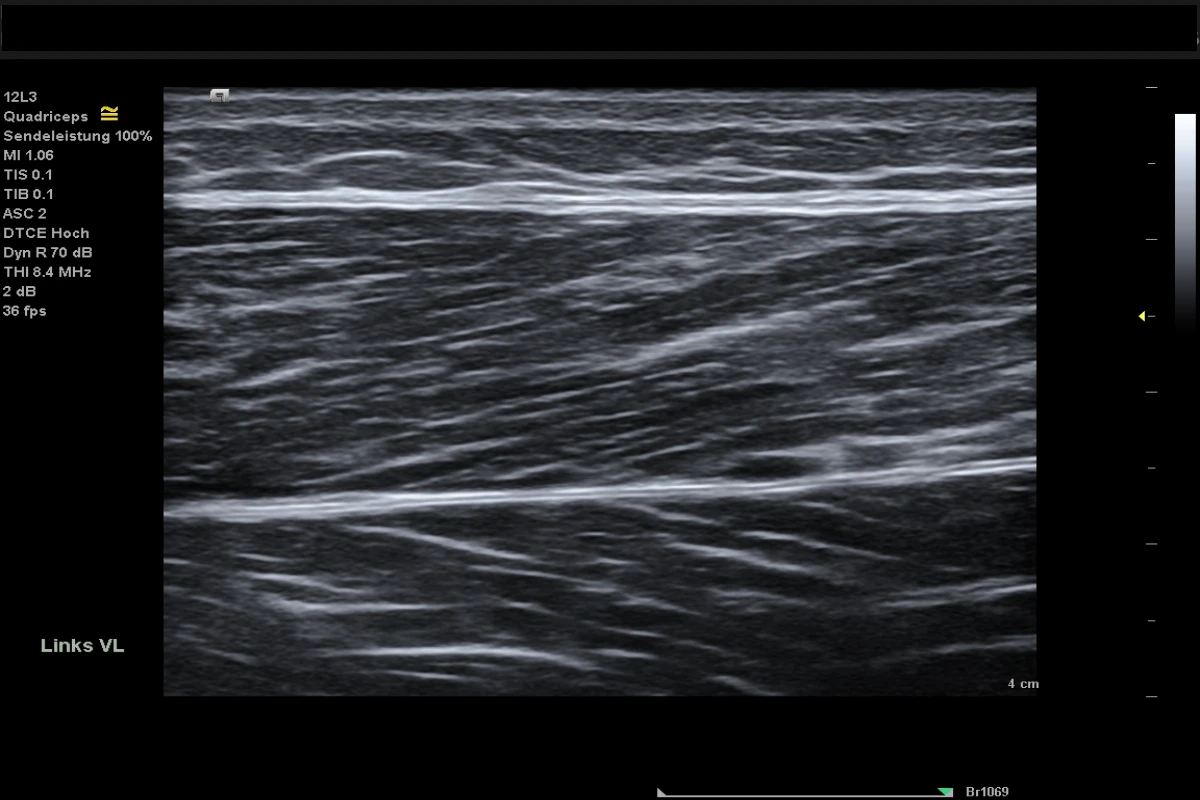
\includegraphics[width=0.46\textwidth]{figures/fig1_raw.png}\hfill
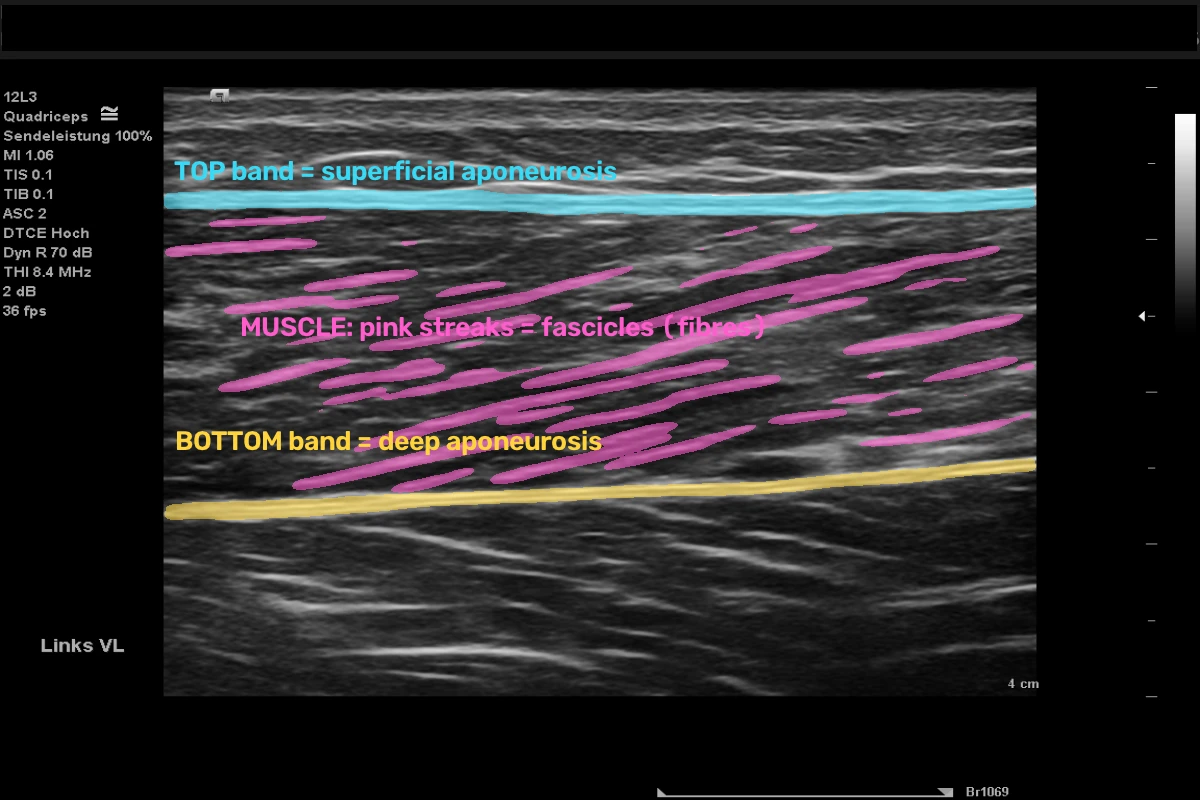
\includegraphics[width=0.46\textwidth]{figures/fig1_annotated.png}
\caption{A longitudinal B-mode image of vastus lateralis as supplied (left) and
with structures indicated (right): the superficial and deep aponeuroses, and
individual fascicles between them. The annotation is illustrative and is not
present in the data. No scale, device identity, or pixel aspect ratio accompanies
the image.}
\label{fig:example}
\end{figure}

Table~\ref{tab:main} and Figure~\ref{fig:comparison} give performance on the
static benchmark. The method scores 0.196 against the seven-rater consensus,
compared with 0.331 for DL\_Track\_US, 0.409 for SMA, and a leave-one-out median
of 0.264 for an individual expert rater. Individual raters span 0.246 to 0.483
leave-one-out; the corresponding mean is 0.303.

\begin{table}[t]
\centering
\caption{Performance on the 35-image static benchmark, all methods scored
against the same seven-rater consensus. Lower is better.}
\label{tab:main}
\begin{tabular}{lcccc}
\toprule
Method & PA ($^{\circ}$) & FL (mm) & MT (mm) & Score \\
\midrule
SMA & 2.39 & 7.01 & 0.74 & 0.409 \\
DL\_Track\_US & 1.45 & 3.74 & 1.31 & 0.331 \\
Single expert (LOO median) & --- & --- & --- & 0.264 \\
\textbf{This method} & \textbf{1.16} & \textbf{2.70} & \textbf{0.51} & \textbf{0.196} \\
\quad on 31 images without training analogues & --- & --- & --- & 0.203 \\
\bottomrule
\end{tabular}
\end{table}

\begin{figure}[t]
\centering
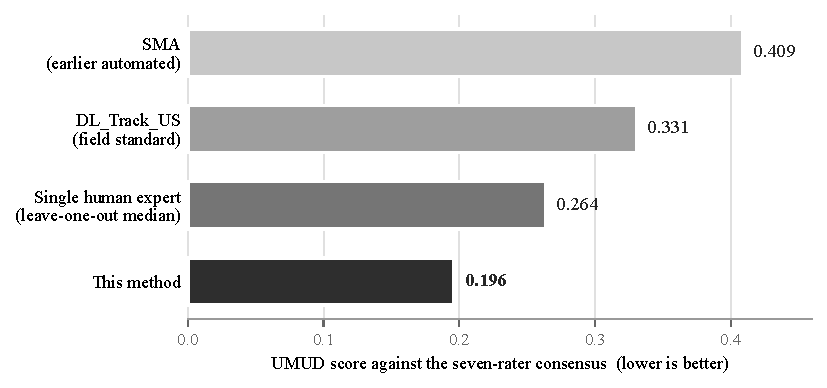
\includegraphics[width=0.82\textwidth]{figures/fig2_comparison.pdf}
\caption{Error against the seven-rater expert consensus on the static benchmark.
Lower values indicate closer agreement.}
\label{fig:comparison}
\end{figure}

Against DL\_Track\_US the present method is more accurate on all three
quantities, and the margin is largest in fascicle length (2.70~mm against
3.74~mm) --- the quantity addressed by Equation~\eqref{eq:fl}. Restricting to 31
benchmark images screened to exclude near-duplicates of training material gives
0.203, bounding residual optimism at approximately 3.5\%.

On the independent dynamic sequence, fascicle-length error is 1.82~mm with the
calibration constant fitted only on the static benchmark, against 2.54~mm
uncalibrated. The earlier fragment-intersection estimator gives 6.45~mm and
3.76~mm respectively. That a constant fitted on one dataset improves a second,
anatomically distinct dataset supports Equation~\eqref{eq:fl} describing a real
geometric effect rather than a fitted artefact.

\section{Discussion}

Two findings merit emphasis. The first is that pixel aspect ratio is not safely
assumed in screenshot-derived ultrasound data. Where an export resamples
horizontally, every angle computed in pixel coordinates is biased, and the
magnitude is substantial: a $12\%$ lateral stretch alters a $20^{\circ}$
pennation angle by more than $2^{\circ}$, which is larger than the inter-rater
disagreement reported here. Because the correction derives from published
aperture specifications, it requires no labelled data and transfers to any
dataset from the same devices.

The second is that the conventional fascicle-length estimator carries a
convergence-dependent bias that human raters do not reproduce.
Equation~\eqref{eq:fl} predicts that this bias should vary between muscles with
differing aponeurosis convergence, which is what we observe ($+8\%$ versus
$+14\%$). The practical consequence is that the fragment estimator requires a
separate calibration per anatomy --- that is, labelled data for every new muscle
--- which defeats the purpose of automation. The bisector form does not.

Several limitations qualify these results. Fascicle segmentation remains the
weakest component (Dice $\approx 0.57$); the geometry stage is deliberately
robust to this through length-weighted voting and outlier rejection, but a
stronger fascicle model is the most direct route to improvement. The residual
calibration constant is empirical: Equation~\eqref{eq:fl} derives the form of
the bias, not its magnitude, and transfer across two datasets is evidence rather
than proof. The benchmark comprises 35 images; all figures use leave-one-out,
but confidence intervals are correspondingly wide and we do not attribute
precise effect sizes to individual components. The anisotropy correction
conflicts with the reference labelling convention on two scanner families, as
set out above. Finally, agreement with a seven-rater consensus is not
anatomical truth --- no biopsy or phantom standard exists for these images --- and
raters may share conventions that an automated method can learn to reproduce.

Device normalisation currently handles six screenshot layouts because those six
were characterised individually; a seventh would require the same treatment.
Automatic recovery of pixel aspect from image content, rather than from a
specification lookup, would remove that constraint and is the natural next step.

\section{Conclusion}

Given only unlabelled ultrasound screenshots from six different devices, a fully
image-computed pipeline estimates muscle architecture more closely to a
seven-rater expert consensus (0.196) than the established open-source tool for
this task (0.331), an earlier automated method (0.409), or an individual expert
rater (0.264). The two components responsible are derived from device optics and
from the geometry of the measurement rather than fitted to the data, which is
why a calibration established on one muscle transfers to another.

\section*{Acknowledgements}

Scanner ruler positions follow the publicly shared analyses ``UMUD Quick and
Dirty'' (AmbrosM) and ``UMUD Pipeline v2'' (Hanh Tran), re-verified against the
images used here.

\section*{Data and code availability}

Evaluation scripts, the model weights, and the split manifests are available at
\url{https://github.com/Cdowning-PDF/umud-muscle-architecture}. The benchmark
datasets are distributed by UMUD \citep{umud2024}.

\begin{thebibliography}{99}
\small

\bibitem[Cronin et al.(2020)]{cronin2020}
Cronin, N.J., Finni, T., Seynnes, O., 2020. Fully automated analysis of muscle
architecture from B-mode ultrasound images with deep learning.
\emph{arXiv:2009.04790}.

\bibitem[He et al.(2016)]{he2016}
He, K., Zhang, X., Ren, S., Sun, J., 2016. Deep residual learning for image
recognition. \emph{Proc. CVPR}, 770--778.

\bibitem[Reliability study(2025)]{frontiers2025}
Reliability of a semi-automated algorithm for muscle architecture analysis,
2025. \emph{Frontiers in Rehabilitation Sciences} 6, 1539804.

\bibitem[Ritsche et al.(2022)]{ritsche2022}
Ritsche, P., Seynnes, O., Cronin, N.J., 2022. DL\_Track\_US: automatic analysis
of longitudinal muscle ultrasonography images. Software.
\url{https://github.com/PaulRitsche/DL\_Track\_US}.

\bibitem[Ritsche et al.(2024)]{ritsche2024}
Ritsche, P., et al., 2024. Fully automated analysis of muscle architecture from
B-mode ultrasound images with DL\_Track\_US. \emph{Ultrasound in Medicine and
Biology}.

\bibitem[Ronneberger et al.(2015)]{ronneberger2015}
Ronneberger, O., Fischer, P., Brox, T., 2015. U-Net: convolutional networks for
biomedical image segmentation. \emph{Proc. MICCAI}, 234--241.

\bibitem[Tan and Le(2019)]{tan2019}
Tan, M., Le, Q.V., 2019. EfficientNet: rethinking model scaling for
convolutional neural networks. \emph{Proc. ICML}, PMLR 97, 6105--6114.

\bibitem[UMUD(2024)]{umud2024}
Ritsche, P., Sarto, F., et al., 2026. UMUD: a web application for easy access to
musculoskeletal ultrasonography datasets. \emph{BMC Medical Imaging}.

\end{thebibliography}

\end{document}
